\section*{Section 1 Parameterized curves}

\begin{tcolorbox}
\section*{第1节 参数曲线}
\end{tcolorbox}

There are two ways to view a curve. Imagine you register for a mountain bike race. The race track, as marked by the organizers, exists independently of you and is described by a certain set of points in space. This one-dimensional object is what we call a curve. However, as a participant in the race, you experience the curve differently: you move along it, and your position can be recorded at different times. This function, which maps time to your position in space, is what we refer to as a parameterized curve.

\begin{tcolorbox}
观察一条曲线有两种方式。想象你报名参加一场山地自行车比赛。比赛路线由组织者标记，独立于你存在，并由空间中的一组点描述。这一维对象我们称为曲线。然而，作为比赛的参与者，你对曲线的体验不同:你沿着它移动，你的位置可以在不同时间被记录。这一函数，将时间映射到你在空间中的位置，我们称之为参数化曲线。
\end{tcolorbox}

\HRule

Definition 1

\begin{tcolorbox}
定义1
\end{tcolorbox}

(Curve)

\begin{tcolorbox}
(曲线)
\end{tcolorbox}

\HRule

A parameterized curve is a smooth map \(c : I \rightarrow  {\mathbb{R}}^{n}\left( {n = 2,3}\right)\) , where \(I\) is an interval, usually \(\left\lbrack  {a,b}\right\rbrack\) or(0,1). A curve is the image of a parameterized curve, i.e., the set \(\{ c\left( t\right)  : t \in  I\}\) .

\begin{tcolorbox}
参数化曲线是一个光滑映射 \(c : I \rightarrow  {\mathbb{R}}^{n}\left( {n = 2,3}\right)\) ，其中 \(I\) 是一个区间，通常为 \(\left\lbrack  {a,b}\right\rbrack\) 或(0,1)。一条曲线是参数化曲线的像，即集合 \(\{ c\left( t\right)  : t \in  I\}\) 。
\end{tcolorbox}

Note that the parameter \(t\) does not necessarily represent time; it can be any parameter that varies along the curve. For example, in the case of the bike race, \(t\) could represent the distance traveled along the track instead of the time elapsed. Nonetheless, it is often convenient to think of \(t\) as time, as it provides an intuitive way to understand the motion along the curve. In this spirit, we refer to \(\dot{c}\left( t\right)  = \frac{\mathrm{d}c}{\mathrm{\;d}t}\) as the velocity vector and \(\ddot{c}\left( t\right)  = \frac{\mathrm{d}\dot{c}}{\mathrm{\;d}t}\) as the acceleration vector.

\begin{tcolorbox}
注意，参数 \(t\) 不一定代表时间；它可以是沿曲线变化的任何参数。例如，在自行车比赛中， \(t\) 可以代表沿路线行驶的距离，而非经过的时间。尽管如此，将 \(t\) 视为时间通常更方便，因为它提供了一种直观理解沿曲线运动的方式。在这种思想下，我们将 \(\dot{c}\left( t\right)  = \frac{\mathrm{d}c}{\mathrm{\;d}t}\) 称为速度向量，将 \(\ddot{c}\left( t\right)  = \frac{\mathrm{d}\dot{c}}{\mathrm{\;d}t}\) 称为加速度向量。
\end{tcolorbox}

There are many different parameterizations for the same curve. For example, different riders may travel at different speeds, leading to different parameterizations of the same physical curve. So we need a way to pass from one parameterization to another.

\begin{tcolorbox}
对于同一条曲线，有许多不同的参数化方式。例如，不同的骑手可能以不同的速度行驶，导致同一物理曲线的不同参数化。因此，我们需要一种方法，将一种参数化转换为另一种参数化。
\end{tcolorbox}

\HRule

Definition 2 (Diffeomorphism)

\begin{tcolorbox}
定义2(微分同胚)
\end{tcolorbox}

\HRule

A smooth map \(\varphi  : {I}_{2} \rightarrow  {I}_{1}\) is called a diffeomorphism if \(\varphi\) is bijective (one-to-one and onto) and its inverse \({\varphi }^{-1}\) is also smooth.

\begin{tcolorbox}
如果光滑映射 \(\varphi  : {I}_{2} \rightarrow  {I}_{1}\) 是双射(既单射又满射)，且其逆映射 \({\varphi }^{-1}\) 也是光滑的，则称 \(\varphi  : {I}_{2} \rightarrow  {I}_{1}\) 为微分同胚。
\end{tcolorbox}

\HRule

Definition 3

\begin{tcolorbox}
定义3
\end{tcolorbox}

(Reparameter-ization)

\begin{tcolorbox}
(重新参数化)
\end{tcolorbox}

\HRule

If \(\varphi  : {I}_{2} \rightarrow  {I}_{1}\) is a diffeomorphism with \({}^{a}{\varphi }^{\prime }\left( t\right)  > 0\) and \({c}_{1} : {I}_{1} \rightarrow  {\mathbb{R}}^{n}\) is a parameterized curve, then \({c}_{2}\left( t\right)  = {c}_{1}\left( {\varphi \left( t\right) }\right)  : {I}_{2} \rightarrow  {\mathbb{R}}^{n}\) is also a parameterized curve, called the reparameterization of \({c}_{1}\) by \(\varphi\) .

\begin{tcolorbox}
如果 \(\varphi  : {I}_{2} \rightarrow  {I}_{1}\) 是一个具有 \({}^{a}{\varphi }^{\prime }\left( t\right)  > 0\) 和 \({c}_{1} : {I}_{1} \rightarrow  {\mathbb{R}}^{n}\) 的微分同胚，且 \({c}_{2}\left( t\right)  = {c}_{1}\left( {\varphi \left( t\right) }\right)  : {I}_{2} \rightarrow  {\mathbb{R}}^{n}\) 是一个参数化曲线，则 \({c}_{1}\) 的重新参数化由 \(\varphi\) 定义，也是一条参数化曲线，称为 \({c}_{1}\) 通过 \(\varphi\) 的重新参数化。
\end{tcolorbox}

\({}^{a}\) A diffeomorphism \(\varphi\) always has either \({\varphi }^{\prime }\left( t\right)  > 0\) or \({\varphi }^{\prime }\left( t\right)  < 0\) for all \(t\) . The latter case would correspond to reversing the direction of the curve.

\begin{tcolorbox}
\({}^{a}\) 一个微分同胚 \(\varphi\) 总是对所有 \(t\) 具有 \({\varphi }^{\prime }\left( t\right)  > 0\) 或 \({\varphi }^{\prime }\left( t\right)  < 0\) 。后者的情况对应于反转曲线的方向。
\end{tcolorbox}

We will often introduce a certain property of the curve using a parameterization, and then show that this property does not depend on the choice of parameterization. For example, the length of a curve is a property that should be independent of how we parameterize it - all riders should better agree on the length of the track, regardless of their speed.

\begin{tcolorbox}
我们经常会用参数化引入曲线的某些性质，然后证明这些性质不依赖于参数化的选择。例如，曲线的长度是一个应当与参数化方式无关的性质——所有骑手都应对轨道的长度达成一致，而不管他们的速度如何。
\end{tcolorbox}

\HRule

Definition 4 (Length of a curve)

\begin{tcolorbox}
定义4(曲线的长度)
\end{tcolorbox}

\HRule

The length of a parameterized curve \(c : I \rightarrow  {\mathbb{R}}^{n}\) is defined as

\begin{tcolorbox}
参数化曲线 \(c : I \rightarrow  {\mathbb{R}}^{n}\) 的长度定义为
\end{tcolorbox}

\[
L\left( c\right)  \mathrel{\text{ := }} {\int }_{a}^{b}\parallel \dot{c}\left( t\right) \parallel \mathrm{d}t \tag{1.1}
\]

where \(I = \left\lbrack  {a,b}\right\rbrack\) or(a, b).

\begin{tcolorbox}
其中 \(I = \left\lbrack  {a,b}\right\rbrack\) 或(a, b)。
\end{tcolorbox}

Lemma 1 | If \({c}_{2}\) is a reparameterization of \({c}_{1}\) , then the length of \({c}_{1}\) and \({c}_{2}\) are the same.

\begin{tcolorbox}
引理1 | 如果 \({c}_{2}\) 是 \({c}_{1}\) 的重新参数化，那么 \({c}_{1}\) 和 \({c}_{2}\) 的长度相同。
\end{tcolorbox}

Proof Since \({c}_{2}\left( t\right)  = {c}_{1}\left( {\varphi \left( t\right) }\right)\) for some diffeomorphism \(\varphi  : {I}_{2} \rightarrow  {I}_{1}\) , we have by the chain rule

\begin{tcolorbox}
证明:由于 \({c}_{2}\left( t\right)  = {c}_{1}\left( {\varphi \left( t\right) }\right)\) 是某个微分同胚 \(\varphi  : {I}_{2} \rightarrow  {I}_{1}\) 的参数化，我们根据链式法则得出
\end{tcolorbox}

\[
{\left. \frac{\mathrm{d}}{\mathrm{d}t}\right| }_{t}{c}_{2} = {\left. {\varphi }^{\prime }\left( t\right) \frac{\mathrm{d}}{\mathrm{d}s}\right| }_{\varphi \left( t\right) }{c}_{1}.
\]

Assume, without loss of generality, that \({I}_{1} = \left\lbrack  {{a}_{1},{b}_{1}}\right\rbrack\) and \({I}_{2} = \left\lbrack  {{a}_{2},{b}_{2}}\right\rbrack\) with \(\varphi \left( {a}_{2}\right)  = {a}_{1}\) and \(\varphi \left( {b}_{2}\right)  = {b}_{1}\) . Thus,

\begin{tcolorbox}
假设，毫无损失地， \({I}_{1} = \left\lbrack  {{a}_{1},{b}_{1}}\right\rbrack\) 和 \({I}_{2} = \left\lbrack  {{a}_{2},{b}_{2}}\right\rbrack\) 具有 \(\varphi \left( {a}_{2}\right)  = {a}_{1}\) 和 \(\varphi \left( {b}_{2}\right)  = {b}_{1}\) 。因此，
\end{tcolorbox}

\[
L\left( {c}_{2}\right)  = {\int }_{{a}_{2}}^{{b}_{2}}\begin{Vmatrix}{{\left. \frac{\mathrm{d}}{\mathrm{d}t}\right| }_{t}{c}_{2}}\end{Vmatrix}\mathrm{d}t
\]

\[
= {\int }_{{a}_{2}}^{{b}_{2}}\left| {{\varphi }^{\prime }\left( t\right) }\right|  \cdot  \begin{Vmatrix}{{\left. \frac{\mathrm{d}}{\mathrm{d}s}\right| }_{\varphi \left( t\right) }{c}_{1}}\end{Vmatrix}\mathrm{d}t
\]

\[
s = \underline{\underline{\varphi }}\left( t\right) {\int }_{{a}_{1}}^{{b}_{1}}{\begin{Vmatrix}{\left. \frac{\mathrm{d}}{\mathrm{d}s}\right| }_{s}{c}_{1}\end{Vmatrix}}_{a}{ds}
\]

\[
= L\left( {c}_{1}\right) ,
\]

where we used the reparameterization theorem for integrals in the third step.

\begin{tcolorbox}
在第三步中，我们使用了积分的重新参数化定理。
\end{tcolorbox}

The proof exhibits a general strategy that we will use often in this course: when we want to investigate a certain property of a curve or surface, we will use a parameterization to boil it down to a problem in calculus that we know how to solve. Here, we just used the chain rule and the reparameterization theorem for integrals.

\begin{tcolorbox}
该证明展示了一种我们在本课程中经常使用的通用策略:当我们想要研究某条曲线或曲面的某个性质时，我们会利用参数化将其简化为我们知道如何解决的微积分问题。在这里，我们只用了链式法则和积分的重新参数化定理。
\end{tcolorbox}

At this point, a word of caution is in order. In the definition of a curve, we required the parameterization to be smooth (i.e, all derivatives exist and are continuous). However, this does not imply that the curve itself is smooth in a geometric sense. For example, the parameterization \(c\left( t\right)  = \left( {{t}^{3},{t}^{2}}\right)\) is smooth, but the curve it describes has a cusp at the origin.

\begin{tcolorbox}
此时，需要提醒一句。在曲线的定义中，我们要求参数化是光滑的(即所有导数存在且连续)。然而，这并不意味着曲线本身在几何意义上是光滑的。例如，参数化 \(c\left( t\right)  = \left( {{t}^{3},{t}^{2}}\right)\) 是光滑的，但它所描述的曲线在原点处有一个尖点(cusp)。
\end{tcolorbox}

\begin{center}
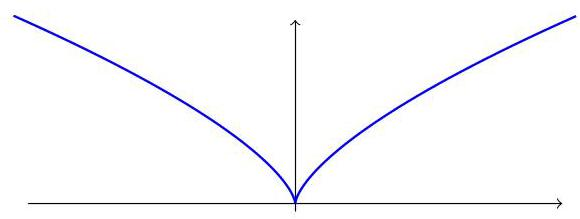
\includegraphics[width=0.4\textwidth]{fig/bo_d3cgcuc601uc738c0ulg_1_462_1366_580_219_0.jpg}
\end{center}
\hspace*{3em} 

Figure 1. Plot of the smooth curve \(c\left( t\right)  = \left( {{t}^{3},{t}^{2}}\right)\) showing a cusp at the origin.

\begin{tcolorbox}
图1。光滑曲线 \(c\left( t\right)  = \left( {{t}^{3},{t}^{2}}\right)\) 的绘图，显示在原点处有一个尖点。
\end{tcolorbox}

To avoid such singularities, we introduce the following definition.

\begin{tcolorbox}
为了避免此类奇异点，我们引入以下定义。
\end{tcolorbox}

\HRule

Definition 5

\begin{tcolorbox}
定义5
\end{tcolorbox}

(Regular curve)

\begin{tcolorbox}
(正则曲线)
\end{tcolorbox}

\HRule

A parameterized curve \(c\) is called regular if \(\dot{c}\left( t\right)  \neq  0\) for all \(t \in  I\) . Such a curve, in particular, has no cusps or corners.

\begin{tcolorbox}
参数化曲线 \(c\) 若对于所有 \(t \in  I\) ，都有 \(\dot{c}\left( t\right)  \neq  0\) ，则称为正则曲线。此类曲线，特别地，没有尖点或角点。
\end{tcolorbox}

The regularity condition ensures that the curve has a well-defined, non-zero tangent vector at every point, which is crucial for many applications in differential geometry. We will almost always assume that the curves we work with are regular. The following result shows that every regular curve can be reparameterized to have unit speed, which is often a convenient choice.

\begin{tcolorbox}
正则性条件确保曲线在每一点都具有良定义的非零切向量，这在微分几何的许多应用中至关重要。我们几乎总是假设所研究的曲线是正则的。以下结果表明，每条正则曲线都可以重新参数化为单位速度的曲线，这通常是一个方便的选择。
\end{tcolorbox}

Proposition 1 For every regular curve \(c : I \rightarrow  {\mathbb{R}}^{n}\) , there exists a diffeomorphism \(\varphi  : I \rightarrow  I\) such that \(\widetilde{c}\left( s\right)  = c\left( {\varphi \left( s\right) }\right)\) has unit-speed, i.e., \(\parallel \dot{\widetilde{c}}\left( s\right) \parallel  = 1\) for all \(s \in  I\) .

\begin{tcolorbox}
命题1:对于每条正则曲线 \(c : I \rightarrow  {\mathbb{R}}^{n}\) ，存在一个微分同胚 \(\varphi  : I \rightarrow  I\) ，使得 \(\widetilde{c}\left( s\right)  = c\left( {\varphi \left( s\right) }\right)\) 具有单位速度，即对于所有 \(s \in  I\) ，有 \(\parallel \dot{\widetilde{c}}\left( s\right) \parallel  = 1\) 。
\end{tcolorbox}

A curve \(c\left( t\right)\) with unit-speed is also called an arc-length parameterization of the curve, since the parameter \(t\) directly measures the length along the curve from some starting point. Indeed, if we let \(l\left( t\right)  = {\int }_{{t}_{0}}^{t}\parallel \dot{c}\left( \tau \right) \parallel \mathrm{d}\tau\) be the length of the arc from a given point \(c\left( {t}_{0}\right)\) to \(c\left( t\right)\) , then for a unit-speed curve, we have \(l\left( t\right)  = t - {t}_{0}\) .

\begin{tcolorbox}
具有单位速度的曲线 \(c\left( t\right)\) 也被称为弧长参数化，因为参数 \(t\) 直接测量沿曲线从某个起点到当前点的长度。实际上，如果让 \(l\left( t\right)  = {\int }_{{t}_{0}}^{t}\parallel \dot{c}\left( \tau \right) \parallel \mathrm{d}\tau\) 表示从某一点 \(c\left( {t}_{0}\right)\) 到 \(c\left( t\right)\) 的弧长，那么对于单位速度的曲线，我们有 \(l\left( t\right)  = t - {t}_{0}\) 。
\end{tcolorbox}

For a unit-speed curve, the velocity vector \(\dot{c}\left( t\right)\) has unit length by definition. We can use the acceleration to find a second vector \(N\left( t\right)\) that is perpendicular to \(\dot{c}\left( t\right)\) and also has unit length.

\begin{tcolorbox}
对于单位速度的曲线，速度向量 \(\dot{c}\left( t\right)\) 的长度由定义即为1。我们可以利用加速度找到第二个向量 \(N\left( t\right)\) ，它与 \(\dot{c}\left( t\right)\) 垂直且也具有单位长度。
\end{tcolorbox}

\HRule

Theorem 1 (Moving frame)

\begin{tcolorbox}
定理1(运动框架)
\end{tcolorbox}

\HRule

Let \(c : I \rightarrow  {\mathbb{R}}^{n}\) be a unit-speed curve with \(\ddot{c}\left( t\right)  \neq  0\) for all \(t\) , then

\begin{tcolorbox}
设 \(c : I \rightarrow  {\mathbb{R}}^{n}\) 是一条单位速度曲线，且对于所有 \(t\) ， \(\ddot{c}\left( t\right)  \neq  0\) ，则
\end{tcolorbox}

\[
T\left( t\right)  \mathrel{\text{ := }} \dot{c}\left( t\right) ,\;N\left( t\right)  \mathrel{\text{ := }} \frac{\ddot{c}\left( t\right) }{\parallel \ddot{c}\left( t\right) \parallel } \tag{1.2}
\]

have unit length and are perpendicular to each other, i.e., they form a pair of orthonormal vectors.

\begin{tcolorbox}
具有单位长度且彼此垂直，即它们形成一对正交归一向量。
\end{tcolorbox}

If the curve lies in \({\mathbb{R}}^{2}\) , then we get two orthonormal vectors \(T\left( t\right)\) and \(N\left( t\right)\) that span \({\mathbb{R}}^{2}\) , i.e., an orthonormal basis of \({\mathbb{R}}^{2}\) that moves along the curve. This is called a moving or Frenet-Serret frame along the curve.

\begin{tcolorbox}
如果该曲线位于 \({\mathbb{R}}^{2}\) 中，则可以得到两个正交归一向量 \(T\left( t\right)\) 和 \(N\left( t\right)\) ，它们张成 \({\mathbb{R}}^{2}\) ，即沿曲线移动的正交归一基底。这被称为沿曲线的运动或弗雷内-塞雷(Frenet-Serret)框架。
\end{tcolorbox}

\HRule

Definition 6 (Curvature)

\begin{tcolorbox}
定义6(曲率)
\end{tcolorbox}

\HRule

The curvature of a unit-speed curve \(c : I \rightarrow  {\mathbb{R}}^{n}\) is defined as \(\kappa \left( t\right)  = \parallel \ddot{c}\left( t\right) \parallel\) .

\begin{tcolorbox}
单位速度曲线 \(c : I \rightarrow  {\mathbb{R}}^{n}\) 的曲率定义为 \(\kappa \left( t\right)  = \parallel \ddot{c}\left( t\right) \parallel\) 。
\end{tcolorbox}

What is the curvature of a general regular curve \(c : I \rightarrow  {\mathbb{R}}^{n}\) ? The natural definition is to first reparameterize \(c\) to a unit-speed curve \(\widetilde{c}\) by a suitable reparameterization \(\varphi\) and then define the curvature of \(c\) as the curvature of \(\widetilde{c}\) . One has to be a bit careful here to measure the curvature at the same point on the curve: If \(c\left( t\right)\) is a point on the curve, then \(\widetilde{c}\left( s\right)  = c\left( {\varphi \left( s\right) }\right)\) is the same point if \(s = {\varphi }^{-1}\left( t\right)\) . Accordingly, we define the curvature \(\kappa \left( t\right)\) of \(c\) at \(t \in  I\) as the curvature \(\widetilde{\kappa }\left( s\right)\) of \(\widetilde{c}\) at \(s = {\varphi }^{-1}\left( t\right)\) , i.e.,

\begin{tcolorbox}
一般正则曲线 \(c : I \rightarrow  {\mathbb{R}}^{n}\) 的曲率是多少？自然的定义是，首先通过适当的参数变换 \(\varphi\) 将 \(c\) 重新参数化为单位速度曲线 \(\widetilde{c}\) ，然后将 \(c\) 的曲率定义为 \(\widetilde{c}\) 的曲率。在这里需要注意的是，要在曲线的同一点测量曲率:如果 \(c\left( t\right)\) 是曲线上的一点，则 \(\widetilde{c}\left( s\right)  = c\left( {\varphi \left( s\right) }\right)\) 也是同一点，如果 \(s = {\varphi }^{-1}\left( t\right)\) 。因此，我们定义在 \(t \in  I\) 处的 \(c\) 的曲率 \(\kappa \left( t\right)\) 为在 \(s = {\varphi }^{-1}\left( t\right)\) 处的 \(\widetilde{c}\) 的曲率 \(\widetilde{\kappa }\left( s\right)\) ，即
\end{tcolorbox}

\[
\kappa \left( t\right)  = \widetilde{\kappa }\left( {{\varphi }^{-1}\left( t\right) }\right) . \tag{1.3}
\]

Lemma 2 If \(c : I \rightarrow  {\mathbb{R}}^{n}\) is a regular curve, then its curvature is given by

\begin{tcolorbox}
引理2:如果 \(c : I \rightarrow  {\mathbb{R}}^{n}\) 是一条正则曲线，则其曲率由以下公式给出
\end{tcolorbox}

\[
\kappa \left( t\right)  = \frac{1}{v{\left( t\right) }^{2}}\sqrt{\parallel \ddot{c}\left( t\right) {\parallel }^{2} - \dot{v}{\left( t\right) }^{2}} = \frac{\sqrt{v{\left( t\right) }^{2}\parallel \ddot{c}\left( t\right) {\parallel }^{2} - {\left( \dot{c}\left( t\right)  \cdot  \ddot{c}\left( t\right) \right) }^{2}}}{v{\left( t\right) }^{3}}, \tag{1.4}
\]

where \(v\left( t\right)  = \parallel \dot{c}\left( t\right) \parallel\) is the speed of \(c\) at time \(t\) .

\begin{tcolorbox}
其中 \(v\left( t\right)  = \parallel \dot{c}\left( t\right) \parallel\) 是 \(c\) 在时间 \(t\) 的速度。
\end{tcolorbox}

\section*{Proof | Homework.}

\begin{tcolorbox}
\section*{证明 | 作业。}
\end{tcolorbox}

The 1-order approximation of a curve is tangent line, while the 2-order approximation is osculating circle.

\begin{tcolorbox}
曲线的一阶近似是切线，而二阶近似是切线圆(拟合圆)。
\end{tcolorbox}

SECTION 2

\section*{Moon in the puddle}

\begin{tcolorbox}
水坑中的月亮
\end{tcolorbox}

One of the overarching themes in differential geometry is to understand how local properties of a curve or surface relate to its global structure. The theorem about the Moon in a puddle is a beautiful example of this idea. It answers the question: If a curve is not too tightly curved, what can we say about the region it encloses?

\begin{tcolorbox}
微分几何中的一个核心主题是理解曲线或曲面局部性质与其整体结构之间的关系。关于水坑中的月亮的定理是这一思想的一个精彩例子。它回答了这样一个问题:如果一条曲线的弯曲不太剧烈，我们可以对它所包围的区域说些什么？
\end{tcolorbox}

To understand the theorem, we first need to introduce a few concepts.

\begin{tcolorbox}
为了理解这个定理，我们首先需要引入一些概念。
\end{tcolorbox}

\HRule

Definition 7 (Loop)

\begin{tcolorbox}
定义7(环)
\end{tcolorbox}

\HRule

A parameterized curve \(c : \left\lbrack  {a,b}\right\rbrack   \rightarrow  {\mathbb{R}}^{n}\) is called a loop if \(c\left( a\right)  = c\left( b\right)\) and all (one-sided) derivatives of \(c\) agree at \(a\) and \(b\) , i.e., \({\left. \frac{{\mathrm{d}}^{k}}{\mathrm{\;d}{t}^{k}}\right| }_{t = a}c\left( t\right)  = {\left. \frac{{\mathrm{d}}^{k}}{\mathrm{\;d}{t}^{k}}\right| }_{t = b}c\left( t\right)\) for all \(k \geq  1\) . It is called simple if it does not intersect itself, i.e., \(c\left( {t}_{1}\right)  \neq  c\left( {t}_{2}\right)\) for all \({t}_{1},{t}_{2} \in  \left( {a,b}\right)\) with \({t}_{1} \neq  {t}_{2}\) .

\begin{tcolorbox}
参数化曲线 \(c : \left\lbrack  {a,b}\right\rbrack   \rightarrow  {\mathbb{R}}^{n}\) 如果 \(c\left( a\right)  = c\left( b\right)\) ，且在 \(a\) 和 \(b\) 处， \(c\) 的所有(单边)导数都一致，即对于所有 \(k \geq  1\) ， \({\left. \frac{{\mathrm{d}}^{k}}{\mathrm{\;d}{t}^{k}}\right| }_{t = a}c\left( t\right)  = {\left. \frac{{\mathrm{d}}^{k}}{\mathrm{\;d}{t}^{k}}\right| }_{t = b}c\left( t\right)\) ，则称为环。如果它不与自身相交，即对于所有 \({t}_{1},{t}_{2} \in  \left( {a,b}\right)\) 和 \({t}_{1} \neq  {t}_{2}\) ， \(c\left( {t}_{1}\right)  \neq  c\left( {t}_{2}\right)\) ，都不相交，则称为简单环。
\end{tcolorbox}

\HRule

Theorem 2 (Jordan curve theorem)

\begin{tcolorbox}
定理2(乔丹曲线定理)
\end{tcolorbox}

\HRule

Every simple loop in \({\mathbb{R}}^{2}\) divides \({\mathbb{R}}^{2}\) into two sets: one is bounded, called the inside; one is unbounded, called the outside.

\begin{tcolorbox}
在 \({\mathbb{R}}^{2}\) 中的每个简单闭合曲线将 \({\mathbb{R}}^{2}\) 划分为两个集合:一个是有界的，称为内部；一个是无界的，称为外部。
\end{tcolorbox}

A classical result about simple curves is the isoperimetric inequality, which states that among all simple loops with a given length, the circle encloses the largest area.

\begin{tcolorbox}
关于简单曲线的一个经典结果是等周不等式，它指出在所有具有给定长度的简单闭合曲线中，圆所包围的面积最大。
\end{tcolorbox}

\HRule

Theorem 3 (Isoperimetric inequality)

\begin{tcolorbox}
定理3(等周不等式)
\end{tcolorbox}

\HRule

Let \(c : \left\lbrack  {a,b}\right\rbrack   \rightarrow  {\mathbb{R}}^{2}\) be a simple loop in \({\mathbb{R}}^{2}\) of length \(L\) enclosing an area \(A\) , then

\begin{tcolorbox}
设 \(c : \left\lbrack  {a,b}\right\rbrack   \rightarrow  {\mathbb{R}}^{2}\) 是长度为 \(L\) 、包围面积为 \(A\) 的简单闭合曲线，若
\end{tcolorbox}

\[
{4\pi A} \leq  {L}^{2},
\]

with equality if and only if \(c\) is a circle.

\begin{tcolorbox}
当且仅当 \(c\) 为圆时取等号。
\end{tcolorbox}

The isoperimetric inequality is a statement about the relationship between two global properties: the length of a curve and the area it encloses. In contrast, the theorem about the Moon in a puddle is a local-to-global result that connects the local property of curvature to the global property of enclosing a unit disc. The following lemma is the key step in the proof of the theorem.

\begin{tcolorbox}
等周不等式是关于两个全局性质之间关系的陈述:曲线的长度与其包围的面积。相比之下，关于水坑中的月亮的定理是一个从局部到全局的结果，它将曲率的局部性质与包围单位圆盘的全局性质联系起来。以下引理是该定理证明的关键步骤。
\end{tcolorbox}

\HRule

Lemma 3

\begin{tcolorbox}
引理3
\end{tcolorbox}

\HRule

Suppose we have a simple, regular loop \(c : I \rightarrow  {\mathbb{R}}^{2}\) . Then there exists a time \({t}_{0} \in  I\) such that the osculating circle at \(c\left( {t}_{0}\right)\) exists and lies inside of \(c\) .

\begin{tcolorbox}
假设我们有一个简单的、规则的闭合曲线 \(c : I \rightarrow  {\mathbb{R}}^{2}\) 。那么存在一个时刻 \({t}_{0} \in  I\) ，在该时刻，曲线在点 \(c\left( {t}_{0}\right)\) 的切线圆存在并位于 \(c\) 内部。
\end{tcolorbox}

\begin{center}
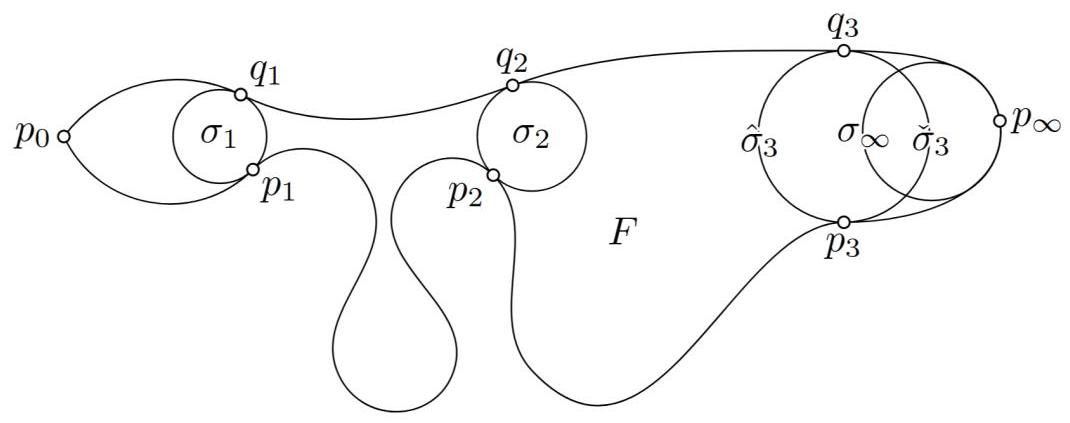
\includegraphics[width=0.8\textwidth]{fig/bo_d3cgcuc601uc738c0ulg_3_224_1244_1070_423_0.jpg}
\end{center}
\hspace*{3em} 

Figure 2. Note that maximal circle \({C}_{p}\) at \(p\) has to touch loop \(c\) at another point \(q\) , but for \({C}_{{p}_{\infty }},{q}_{\infty } = {p}_{\infty } -\) a contradiction.

\begin{tcolorbox}
图2。注意，在点 \(p\) 处的最大圆 \({C}_{p}\) 必须与曲线 \(c\) 在另一点 \(q\) 相切，但对于 \({C}_{{p}_{\infty }},{q}_{\infty } = {p}_{\infty } -\) 来说，这是一个矛盾。
\end{tcolorbox}

\HRule

Theorem 4 ("Moon in the puddle")

\begin{tcolorbox}
定理4(“水坑中的月亮”)
\end{tcolorbox}

\HRule

Let \(c : I \rightarrow  {\mathbb{R}}^{2}\) be a simple, regular loop. If \(\kappa \left( t\right)  \leq  1\) for all \(t \in  I\) , then the region surrounded by \(c\) contains a unit disc.

\begin{tcolorbox}
设 \(c : I \rightarrow  {\mathbb{R}}^{2}\) 为一个简单、规则的闭合曲线。如果对于所有 \(t \in  I\) ，都满足 \(\kappa \left( t\right)  \leq  1\) ，那么由 \(c\) 包围的区域包含一个单位圆盘。
\end{tcolorbox}

Proof | By the lemma, there exists a point \(p = c\left( {t}_{0}\right)\) on the curve such that the osculating circle \(\sigma\) at \(p\) lies inside of \(c\) . But \(\sigma\) has radius \(r = 1/\kappa \left( {t}_{0}\right)  \geq  1\) , so it contains a unit disc.

\begin{tcolorbox}
证明| 根据引理，存在曲线上的一点 \(p = c\left( {t}_{0}\right)\) ，在该点的切线圆 \(\sigma\) 位于 \(c\) 内部。但 \(\sigma\) 的半径为 \(r = 1/\kappa \left( {t}_{0}\right)  \geq  1\) ，因此它包含一个单位圆盘。
\end{tcolorbox}

\section*{Winding number}

\begin{tcolorbox}
\section*{绕数}
\end{tcolorbox}

Another common theme in differential geometry is that the integral of a local quantity over a closed curve or surface often yields a discrete global invariant of the object.

\begin{tcolorbox}
微分几何中的另一个常见主题是，局部量在闭合曲线或曲面上的积分常常产生对象的离散全局不变量。
\end{tcolorbox}

For example, consider a simple loop \(c : \left\lbrack  {a,b}\right\rbrack   \rightarrow  {\mathbb{R}}^{2}\) in the plane that does not pass through the origin. Then we can look at the expression

\begin{tcolorbox}
例如，考虑平面中的一个不经过原点的简单闭合曲线 \(c : \left\lbrack  {a,b}\right\rbrack   \rightarrow  {\mathbb{R}}^{2}\) 。然后我们可以观察表达式
\end{tcolorbox}

\[
\frac{1}{2\pi }{\int }_{a}^{b}\frac{x\left( t\right) \dot{y}\left( t\right)  - y\left( t\right) \dot{x}\left( t\right) }{x{\left( t\right) }^{2} + y{\left( t\right) }^{2}}\mathrm{\;d}t. \tag{3.1}
\]

A priori, this integral could take any real value. And you might expect that if you deform the curve slightly, the integrand would change continuously, and thus the value of the integral would also change continuously. However, this is not the case. The integral actually takes on only integer values and remains invariant under continuous deformations of the curve that do not pass through the origin.

\begin{tcolorbox}
先验上，这个积分可以取任何实数值。你可能会预期，如果你稍微变形曲线，被积函数会连续变化，因此积分的值也会连续变化。然而，事实并非如此。这个积分实际上只取整数值，并且在不经过原点的连续变形下保持不变。
\end{tcolorbox}

To understand why this is true, it is helpful to start from the following geometric notion.

\begin{tcolorbox}
为了理解为什么会这样，有助于从以下几何概念入手。
\end{tcolorbox}

\HRule

Definition 8 (Winding number)

\begin{tcolorbox}
定义8(绕数)
\end{tcolorbox}

\HRule

Let \(c : \left\lbrack  {a,b}\right\rbrack   \rightarrow  {\mathbb{R}}^{2}\) be a loop and \({P}_{0}\) be a point that does not lie on the curve. The winding number \(W\left( {c,{P}_{0}}\right)\) is the number of times the curve goes counter-clockwise around \({P}_{0}\) .

\begin{tcolorbox}
设 \(c : \left\lbrack  {a,b}\right\rbrack   \rightarrow  {\mathbb{R}}^{2}\) 为一条闭合曲线， \({P}_{0}\) 为不在曲线上的一点。绕数 \(W\left( {c,{P}_{0}}\right)\) 是曲线逆时针绕 \({P}_{0}\) 的次数。
\end{tcolorbox}

From geometric considerations, it is clear that the winding number is an integer that satisfies the following properties:

\begin{tcolorbox}
从几何角度来看，很明显绕数是一个满足以下性质的整数:
\end{tcolorbox}

\HRule

Proposition 2

\begin{tcolorbox}
命题2
\end{tcolorbox}

\HRule

\begin{itemize}
\item \(W\left( {c,{P}_{0}}\right)\) depends on \({P}_{0}\) ;
\end{itemize}

\begin{tcolorbox}
\begin{itemize}
\item \(W\left( {c,{P}_{0}}\right)\) 依赖于 \({P}_{0}\) ；
\end{itemize}
\end{tcolorbox}

\begin{itemize}
\item \(W\left( {c,{P}_{1}}\right)  = W\left( {c,{P}_{2}}\right)\) if \({P}_{1}\) and \({P}_{2}\) can be connected by a curve not intersecting \(C\) .
\end{itemize}

\begin{tcolorbox}
\begin{itemize}
\item 如果 \({P}_{1}\) 和 \({P}_{2}\) 可以通过一条不与 \(C\) 相交的曲线相连，则 \(W\left( {c,{P}_{1}}\right)  = W\left( {c,{P}_{2}}\right)\) 相同。
\end{itemize}
\end{tcolorbox}

\begin{itemize}
\item \(W\left( {c,{P}_{0}}\right)\) is invariant under continuous deformations of \(c\) that do not pass through \({P}_{0}\) , i.e., if \({c}_{\delta }\) is a family of loops with \({c}_{\delta }\left( t\right)  \neq  {P}_{0}\) for all \(\delta ,t\) , then \(W\left( {{c}_{\delta },{P}_{0}}\right)\) is independent of \(\delta\) .
\end{itemize}

\begin{tcolorbox}
\begin{itemize}
\item 在不经过 \({P}_{0}\) 的连续变形下， \(W\left( {c,{P}_{0}}\right)\) 保持不变，即如果 \({c}_{\delta }\) 是一族满足 \({c}_{\delta }\left( t\right)  \neq  {P}_{0}\) 的闭合曲线，则 \(W\left( {{c}_{\delta },{P}_{0}}\right)\) 与 \(\delta\) 无关。
\end{itemize}
\end{tcolorbox}

To get a formula for the winding number, we first shift the curve so that \({P}_{0}\) is at the origin. Then we can express the curve in polar coordinates \({}^{1}c\left( t\right)  = r\left( t\right) \left( {\cos \theta \left( t\right) ,\sin \theta \left( t\right) }\right)\) with \(r\left( t\right)  > 0\) for all \(t\) . Since the curve is a loop, we have \(r\left( a\right)  = r\left( b\right)\) and \(\theta \left( b\right)  = \theta \left( a\right)  + {2k\pi }\) for some integer \(k\) . Clearly \(k\) is the winding number of \(c\) around the origin. To find a formula for \(k = \frac{\theta \left( b\right)  - \theta \left( a\right) }{2\pi }\) , we will find an expression for \(\dot{\theta }\left( t\right)\) and then integrate it over \(\left\lbrack  {a,b}\right\rbrack\) . Denoting the components of \(c\left( t\right)\) by \(x\left( t\right)\) and \(y\left( t\right)\) , we have

\begin{tcolorbox}
为了得到绕数的公式，首先将曲线平移，使得 \({P}_{0}\) 位于原点。然后可以用极坐标 \({}^{1}c\left( t\right)  = r\left( t\right) \left( {\cos \theta \left( t\right) ,\sin \theta \left( t\right) }\right)\) 表示曲线，其中 \(r\left( t\right)  > 0\) 对所有 \(t\) 成立。由于曲线是闭合的，我们有 \(r\left( a\right)  = r\left( b\right)\) 和 \(\theta \left( b\right)  = \theta \left( a\right)  + {2k\pi }\) ，其中 \(k\) 是某个整数。显然， \(k\) 是 \(c\) 绕原点的绕数。为了找到 \(k = \frac{\theta \left( b\right)  - \theta \left( a\right) }{2\pi }\) 的公式，我们将找到 \(\dot{\theta }\left( t\right)\) 的表达式，然后在 \(\left\lbrack  {a,b}\right\rbrack\) 上对其积分。用 \(c\left( t\right)\) 的分量用 \(x\left( t\right)\) 和 \(y\left( t\right)\) 表示，我们有
\end{tcolorbox}

\[
\left( \begin{array}{l} \dot{x} \\  \dot{y} \end{array}\right)  = \dot{c} = \dot{r}\left( \begin{matrix} \cos \theta \\  \sin \theta  \end{matrix}\right)  + r\dot{\theta }\left( \begin{matrix}  - \sin \theta \\  \cos \theta  \end{matrix}\right)  \tag{3.2}
\]

\[
= \frac{\dot{r}}{r}\left( \begin{array}{l} x \\  y \end{array}\right)  + \dot{\theta }\left( \begin{matrix}  - y \\  x \end{matrix}\right) .
\]

\customfootnote{

\({}^{1}\) Strictly speaking, we view \(\theta\) here as a smooth real-valued function of \(t\) (and not modulo \({2\pi }\) ). This is possible because the polar coordinates furnish a covering map \(\left( {r,\theta }\right)  \mapsto  r\left( {\cos \theta ,\sin \theta }\right)\) from \(\left( {0,\infty }\right)  \times  \mathbb{R}\) to \({\mathbb{R}}^{2} \smallsetminus  \{ 0\}\) . Then, using the lifting property of covering spaces, we can lift the curve \(c\) in \({\mathbb{R}}^{2} \smallsetminus  \{ 0\}\) to a curve in \(\left( {0,\infty }\right)  \times  \mathbb{R}\) , whose coordinates are exactly the functions \(r\left( t\right)\) and \(\theta \left( t\right)\) .

\begin{tcolorbox}
\({}^{1}\) 严格来说，我们将 \(\theta\) 视为关于 \(t\) 的光滑实值函数(而非模 \({2\pi }\) 的函数)。这是可能的，因为极坐标提供了从 \(\left( {0,\infty }\right)  \times  \mathbb{R}\) 到 \({\mathbb{R}}^{2} \smallsetminus  \{ 0\}\) 的覆盖映射 \(\left( {r,\theta }\right)  \mapsto  r\left( {\cos \theta ,\sin \theta }\right)\) 。然后，利用覆盖空间的提升性质，我们可以将 \({\mathbb{R}}^{2} \smallsetminus  \{ 0\}\) 中的曲线 \(c\) 提升到 \(\left( {0,\infty }\right)  \times  \mathbb{R}\) 中的一条曲线，其坐标正是函数 \(r\left( t\right)\) 和 \(\theta \left( t\right)\) 。
\end{tcolorbox}

}

Taking the dot product of both sides with(-y, x), we conclude that

\begin{tcolorbox}
两边取点积与(-y, x)，我们得出结论
\end{tcolorbox}

\[
\dot{\theta } = \frac{x\dot{y} - y\dot{x}}{{x}^{2} + {y}^{2}}. \tag{3.3}
\]

To find the winding number, we can integrate \(\dot{\theta }\) :

\begin{tcolorbox}
为了求绕数(winding number)，我们可以对 \(\dot{\theta }\) 进行积分:
\end{tcolorbox}

\[
W\left( {c,0}\right)  = \frac{\theta \left( b\right)  - \theta \left( a\right) }{2\pi } = \frac{1}{2\pi }{\int }_{a}^{b}\frac{x\dot{y} - y\dot{x}}{{x}^{2} + {y}^{2}}\mathrm{\;d}t. \tag{3.4}
\]

This is exactly the integral we started with!

\begin{tcolorbox}
这正是我们一开始所用的积分！
\end{tcolorbox}

Section 4

\begin{tcolorbox}
第4节
\end{tcolorbox}

Frenet-Serret frames for curves in \({\mathbb{R}}^{3}\)

\begin{tcolorbox}
曲线在 \({\mathbb{R}}^{3}\) 中的弗雷内-塞雷(Frenet-Serret)框架
\end{tcolorbox}

Curves in \({\mathbb{R}}^{3}\) can

\begin{tcolorbox}
在 \({\mathbb{R}}^{3}\) 中的曲线可以
\end{tcolorbox}

\begin{itemize}
\item bend: measured by curvature (how much the curve deviates from being a straight line in a plane)
\end{itemize}

\begin{tcolorbox}
\begin{itemize}
\item 弯曲:由曲率(衡量曲线偏离直线的程度)来测量
\end{itemize}
\end{tcolorbox}

\begin{itemize}
\item twist: measured by torsion (how much this plane rotates along the curve)
\end{itemize}

\begin{tcolorbox}
\begin{itemize}
\item 扭转:由挠率(衡量沿曲线旋转的平面程度)来测量
\end{itemize}
\end{tcolorbox}

\HRule

Definition 9 (Frenet-Serret frame)

\begin{tcolorbox}
定义9(弗雷内-塞雷框架)
\end{tcolorbox}

\HRule

Let \(c\) be a unit-speed curve in \({\mathbb{R}}^{3},T\left( t\right)  = \dot{c}\left( t\right)\) be the tangent field, curvature \(\kappa \left( t\right)  =\)  \(\left| {\ddot{c}\left( t\right) }\right|\) . Assume \(\kappa \left( t\right)  > 0\) , then \(N\left( t\right)  = \frac{\ddot{c}\left( t\right) }{\left| \ddot{c}\left( t\right) \right| }\) , and \(B\left( t\right)  = T\left( t\right)  \times  N\left( t\right)\) is the binormal field. Here \(\{ T,N,B\}\) is called the Frenet-Serret frame.

\begin{tcolorbox}
设 \(c\) 为一条单位速度的曲线， \({\mathbb{R}}^{3},T\left( t\right)  = \dot{c}\left( t\right)\) 为切向场，曲率为 \(\kappa \left( t\right)  =\)  \(\left| {\ddot{c}\left( t\right) }\right|\) 。假设 \(\kappa \left( t\right)  > 0\) ，则 \(N\left( t\right)  = \frac{\ddot{c}\left( t\right) }{\left| \ddot{c}\left( t\right) \right| }\) ，而 \(B\left( t\right)  = T\left( t\right)  \times  N\left( t\right)\) 为二法向场。这里 \(\{ T,N,B\}\) 称为弗雷内-塞雷(Frenet-Serret)框架。
\end{tcolorbox}

\(T\left( t\right) ,N\left( t\right) ,B\left( t\right)\) are orthogonal to each other and have unit length; notice that \(\left| {v \times  w}\right|  =\)  \(\left( {v,v}\right) \left( {w,w}\right)  - {\left( v,w\right) }^{2}\) .

\begin{tcolorbox}
\(T\left( t\right) ,N\left( t\right) ,B\left( t\right)\) 彼此正交且长度为单位；注意 \(\left| {v \times  w}\right|  =\)  \(\left( {v,v}\right) \left( {w,w}\right)  - {\left( v,w\right) }^{2}\) 。
\end{tcolorbox}

\HRule

Theorem 5 (Frenet-Serret equations)

\begin{tcolorbox}
定理5(弗雷内-塞雷方程)
\end{tcolorbox}

\HRule

If \(c : I \rightarrow  {\mathbb{R}}^{3}\) is a unit-speed curve with \(\mathrm{F} - \mathrm{N}\) frame \(T,N,B\) , then

\begin{tcolorbox}
如果 \(c : I \rightarrow  {\mathbb{R}}^{3}\) 是一条单位速度的曲线，且具有 \(\mathrm{F} - \mathrm{N}\) 框架 \(T,N,B\) ，那么
\end{tcolorbox}

\[
\frac{\mathrm{d}}{\mathrm{d}t}\left( \begin{array}{l} T \\  N \\  B \end{array}\right)  = \left( \begin{matrix} 0 & \kappa & 0 \\   - \kappa & 0 & \tau \\  0 &  - \tau & 0 \end{matrix}\right) \left( \begin{array}{l} T \\  N \\  B \end{array}\right)  \tag{4.1}
\]

where \(\tau \left( t\right)  =  - \dot{B}\left( t\right)  \cdot  N\left( t\right)  = \dot{N}\left( t\right)  \cdot  B\left( t\right)\) is called the torsion of \(c\) at \(t\) .

\begin{tcolorbox}
其中 \(\tau \left( t\right)  =  - \dot{B}\left( t\right)  \cdot  N\left( t\right)  = \dot{N}\left( t\right)  \cdot  B\left( t\right)\) 被称为 \(c\) 在 \(t\) 处的挠率(torsion)。
\end{tcolorbox}

Remark The matrix

\begin{tcolorbox}
备注:该矩阵
\end{tcolorbox}

\[
\Omega  = \left( \begin{matrix} 0 & \kappa & 0 \\   - \kappa & 0 & \tau \\  0 &  - \tau & 0 \end{matrix}\right)  \tag{4.2}
\]

tells us how the Frenet-Serret frame changes along the curve. So if \(T,N,B\) are the frame vectors at time \(t\) , then at time \(t + {\Delta t}\) , the frame vectors are approximately

\begin{tcolorbox}
告诉我们弗雷内-塞雷(Frenet-Serret)框架沿曲线的变化情况。因此，如果 \(T,N,B\) 是时间 \(t\) 时的框架向量，那么在时间 \(t + {\Delta t}\) 时，框架向量大致为
\end{tcolorbox}

\[
\left( {1 + {\Delta t\Omega }}\right) \left( \begin{array}{l} T \\  N \\  B \end{array}\right) . \tag{4.3}
\]

The fact that \(\Omega\) is skew-symmetric (i.e., \({\Omega }^{T} =  - \Omega\) ) means that the transformation \(1 + {\Delta t\Omega }\) is an infinitesimal rotation. Geometrically, this means that as we move along the curve, the Frenet-Serret frame rotates in a way that is determined by the curvature and torsion of the curve.

\begin{tcolorbox}
\(\Omega\) 是反对称的(即， \({\Omega }^{T} =  - \Omega\) )，意味着变换 \(1 + {\Delta t\Omega }\) 是一个无穷小旋转。从几何角度来看，这意味着沿着曲线移动时，弗雷内-塞雷(Frenet-Serret)框架会以由曲线的曲率和挠率决定的方式旋转。
\end{tcolorbox}